% Created 2025-09-06 Sat 11:07
% Created 2025-09-06 Sat 11:07
% Intended LaTeX compiler: pdflatex
\documentclass[presentation]{beamer}
\usepackage[utf8]{inputenc}
\usepackage[T1]{fontenc}
\usepackage{amsmath}
\usepackage{amssymb}
\usepackage{capt-of}
\usepackage{hyperref}
\usepackage{lmodern}
\usepackage{fontenc}
\usepackage{inputenc}
\usepackage{amsmath}
\usepackage{amssymb}
\usepackage{mathtools}
\usepackage{bm}
\usepackage{xcolor}
\usepackage{graphicx}

\usetheme{default}
\author{Rasmus Sten}
\date{\today}
\title{Presentation Studieteknik}
\usepackage{hyperref}
\providecolor{url}{HTML}{0077bb}
\providecolor{link}{HTML}{882255}
\providecolor{cite}{HTML}{999933}
\hypersetup{
  pdfauthor={Rasmus Sten},
  pdftitle={Presentation Studieteknik},
  pdfkeywords={},
  pdfsubject={},
  pdfcreator={},
  pdflang={English},
  breaklinks=true,
  colorlinks=true,
  linkcolor=link,
  urlcolor=url,
  citecolor=cite
}
\urlstyle{same}
% Hide link styles in table of contents
\NewCommandCopy{\oldtoc}{\tableofcontents}

\begin{document}

\maketitle
\frametitle{Introduction}
\section{Introduction}
\begin{frame}{Introduktion}
  \note{Presentera dig själv, ta emot frågor, be dem ställa frågor ifall de vill att jag förtydligar något}

  \note{Fråga vad de vill att jag prioriterar}
Presentationens innehåll:
\begin{itemize}
\item Skäl till en god studieteknik
  \item Principer av den personliga studietekniken (som inte täcks av utbildningen)
        \begin{itemize}
          \item Förstå djupet
          \item Fokus
          \item Övning
          \item Förståelse och minne
          \item Intuition
       \end{itemize}

\item Att ta anteckningar
\item Filosofi om och val av mjukvara
\end{itemize}


\note{
Innan jag fortsätter\ldots

  Fråga publiken om hur de känner om sin studieteknik, ta frågor, skriv upp grupper på tavlan.

  Eftersom denna presentation inte är obligatorisk, förväntar jag mig främst två typer av personer här:
  1. De som är medvetna om sina brister.
  2. De som redan är erfarna, men vill lära sig mer.
  Sedan saknar vi säkert många som hade behövt ta del av detta men hellre gör annat.
}

\end{frame}

\begin{frame}{Varför studieteknik?}

\note{Faktumet att ni har valt att närvara antyder att ni placerar ett visst värde i er studieteknik. *Fråga publiken vad de ser som skäl, även om det är uppenbart*}

\begin{itemize}
  \item Tidseffektivitet
\note{Jag önskar ibland att jag pluggade bättre under tidiga kurser, inte mer, utan bättre}
  \item Självsäkerhet, mindre ångest och stress
  \note{Självsäkerhet går att se som en medvetenhet om sin egen skicklighet jämtemot vad som förväntas av en uppgift, därav blir det enklare att plugga när man vet sin egen förmåga}

  \item Roligt att plugga?
  \note{Inte säkert att bioteknik är rätt utbildning för den alla ni är innerst inne, men det kommer ni att få lista ut på egen hand.}
\end{itemize}

\note{
Fråga om de vet vad kostnaden för en icke-EU student att läsa envariabelsanalys 1. \textbf{Avgift för Envariabelsanalys 1 (7,5 hp): 20,000 kr}
Förklara hur samhället placerar en stor vikt vid att studenterna lär sig förstå och använda viktig information: Viss del av kostnaden är för administrativt och för resurser, men en stor måste vi anta är hur informationen lärs ut.}

\textbf{Formell utbildning vs. personlig utbildning}
\begin{itemize}
\item Utbildningsplan, samhällsforsking, duktiga lärare
\item Ordentligt, eget arbete
\note{Det finns däremot delar som de inte kan göra åt oss, vilket är vad denna föreläsning är till för.}
\end{itemize}
\end{frame}


\begin{frame}


\includegraphics[height=0.8\textheight]{images/joshua_graham.png}
\end{frame}

\begin{frame}{Ultralearning}

\note{I mitten av min utbildning läste jag boken Ultralearning av Scott Young, som diskuterar principer för effektiv inlärning. Det är dessa knep som används av personer som lär sig tala flera språk under kort tid, advancerad veteksap, tekniker o.s.v.. Vad jag insåg när jag läste boken var att jag hade behövt lära mig vissa av hans principer den hårda vägen. Jag lärde mig också att flera av principerna täcks väldigt väl av universitetet. Därför har jag inkluderat de delar som inte täcks väl kommer jag kort förklara hur och när jag använder dem}

\begin{itemize}

  \item \textit{Ultralearning} (2019): bok av Scott Young om principer för effektiv inlärning


\item Vad inte formell utbildning inte erbjuder


\item Förstås finns det viktiga aspekter som hur roligt/intressant, svårt eller omfattande materialet är (\href{https://www.youtube.com/watch?v=167se17RNHw}{\textit{The power of interest}})


\item Viktigast inom ultralearning är att förstå \emph{när} man ska använda \emph{vad}
\end{itemize}
\end{frame}

\begin{frame}{Ultralearning 1 - Urskilj detaljnivån}

\textbf{Relevans för tentamen}
\begin{itemize}
    \item Kunskapskrav och kursöversikt på umu.se eller canvas
    \item Studiefrågor eller gamla tentor (Mamma muu har en drive\ldots)
    \item Fråga föreläsaren, särskilt den som skriver tentan
\end{itemize}

\textbf{Relevans för verkligheten}

Fokusera på det som är väsentligt.

Men hur vet du vilka delar av kursen som är väsentliga?

\note{Ni vet sannolikt inte hur arbetslivet ser ut som en biotekniker
  Fråga: vet någon vad en biotekniker gör?
  Det listade jag inte ut förens något år in på utbildningen.}
\end{frame}

\begin{frame}{Ultralearning 1 - Urskilj detaljnivån forts.}

\begin{itemize}
    \item Labbar och tillämpade exempel. Vissa tentafrågor kommer i dessa former.
    \item Att skapa egna praktiska problem att lösa hjälper dig att hitta den verkligen relevanta informationen.
    \item Om du förstår vad du förväntas veta blir det lättare att urskilja vad som är viktigt. Läs kursplanerna. Börja baklänges genom att titta på hur dessa tekniker tillämpas.
    \item Om du har svårt att förstå hur vissa delar av informationen tillämpas, om de ens gör det, kan du be AI skapa tillämpningar inom bioteknik. Exempel på sådana områden är grundläggande teori inom kodning, kalkyl eller kemi.
\end{itemize}

\note{
Personligt exempel: För många tidiga kurser skrev jag ner många detaljer och gjorde mina anteckningar och ekvationer snygga. Det kändes rätt, men det var inte där jag fick störst utdelning för tiden jag spenderade. Jag borde ha fokuserat på information och koncept som hjälpte mig att förstå de förväntade lärandemålen och nöjt mig med det. Under de senare kurserna av utbildningen (år 5) tänkte jag främst på vad jag ville ta med mig för kunskap till arbetslivet.
}

\end{frame}

\begin{frame}{Ultralearning 2 - Fokus}
  För en djupare förståelse, läs \textit{Ultralearning} kapitel~2.

 Young beskriver tre vanliga fallgropar för fokus:
\begin{itemize}
    \item Prokrastinering
    \item Distraktion
    \item Att inte skapa rätt sorts fokus
\end{itemize}

\end{frame}

\begin{frame}{Prokrastinering}
\begin{quote}
“Mycket prokrastinering är omedveten. Att inse att du prokrastinerar är det första steget för att undvika det.”\\
— Scott Young, \textit{Ultralearning}
\end{quote}

Att börja arbeta med något tråkigt är svårt. Varför är det tråkigt?
\begin{itemize}
    \item Du vet inte varför du tycker att du ska göra det. Det är inte bra om det enda skälet är för att klara tentan.
    \item Kontrasten mellan hur roligt studierna är jämfört med fritidsaktiviteter gynnar det senare.
    \item Lösningar? Förstå varför du är i programmet. Justera dopaminbalansen (se \href{https://www.youtube.com/watch?v=8GUNhGRlQDU}{\textit{How To Reprogram Your Dopamine To Crave Hard Work}})
\end{itemize}
\end{frame}

\begin{frame}{Pomodoro-tekniken}
Innan du har bemästrat fokus:
\begin{itemize}
    \item Använd Pomodoro: 25 minuters fokus, följt av 5 minuters paus.
    \item Var strikt med att återgå till arbete när pausen är över.
    \item När du förbättras, förläng studietiden --- men bli inte kaxig och strunta i pausen.
\end{itemize}
Blir du duktig nog på att hålla fokus, kommer detta aldrig att bli ett problem.
\end{frame}

% --- Slide 4: Distraktionskällor (Miljö) ---
\begin{frame}{Distraktioner: Miljö}
Externa faktorer som kan störa fokus:
\begin{itemize}
    \item Studera ensam eller med vänner som delar engagemang.
    \item Sätt telefonen på stör ej, lägg den i ett annat rum.
    \item Samla allt du behöver innan du börjar.
    \item Undvik multitasking: definiera uppgiften innan start.
    \item När du börjar, sluta inte förrän timern är slut.
\end{itemize}
\end{frame}

% --- Slide 5: Distraktionskällor (Uppgift) ---
\begin{frame}{Distraktioner: Uppgift}
\begin{quote}
“Vet att vissa aktiviteter, på grund av deras natur, är svårare att fokusera på än andra.”\\
— Scott Young, \textit{Ultralearning}
\end{quote}

Detta är varför du måste lära dig att tycka om ämnena.
Exempel på utmanande ämnen:
\begin{itemize}
    \item Matematik (särskilt bevis)
    \item Statistiska metoder
    \item Cellsignaleringsvägar
    \item Organiska reagenser och mekanismer
    \item Labbrapporter (vanligt bland nyare studenter)
\end{itemize}
Tips: Läs med ett specifikt syfte – sök efter det du behöver förstå.
\end{frame}

% --- Slide 6: Distraktionskällor (Sinnet) ---
\begin{frame}{Distraktioner: Sinnet}
Negativa känslor, stress, rastlöshet och beroende kan hindra fokus.

För att förbättra:
\begin{itemize}
    \item Sov tillräckligt (8 timmar)
    \item Ät mångsidigt
    \item Rör på dig regelbundet
    \item Var tillräckligt social
    \item Ta bort missbruk
\end{itemize}

Det är okej att överge en studiesession om det är för det större goda --- men var tydligt mot dig själv att du överger uppgiften och släpper den.
\end{frame}

% --- Slide 7: Shallow vs Deep Focus ---
\begin{frame}{Rätt typ av fokus}
\textbf{Shallow focus:}
\begin{quote}
“Icke-kognitivt krävande, logistiska uppgifter …  lätta att replikera.”\\
— Cal Newport, \textit{Deep Work}
\end{quote}

\textbf{Deep focus (flow):}
\begin{quote}
“Professionella aktiviteter utförda i ett tillstånd av distraktionsfri koncentration som driver dina kognitiva förmågor till deras gräns.”\\
— Cal Newport, \textit{Deep Work}
\end{quote}
\end{frame}

% --- Slide 8: Att integrera Deep Work ---
\begin{frame}{Att integrera Deep Work}
För att integrera djupt arbete:
\begin{itemize}
    \item Bestäm var och hur länge du ska arbeta.
    \item Inför regler (t.ex. förbud mot internet) under sessions.
    \item Stöd hjärnan: kaffe, rätt mat, lätt motion.
\end{itemize}
Som Cal Newport skriver: Ritualen måste specificera \emph{var}, \emph{hur}, \emph{hur länge} och \emph{stöd}.
\end{frame}

% --- Slide 9: Förbättra fokus ---
\begin{frame}{Förbättra fokus}
Du kan öva din förmåga att fokusera genom att hålla kvar tankar under ledig tid.
Ju längre du kan hålla en enda tanke utan att bli distraherad, desto bättre fokus kommer du att ha.

\note{
Personligt exempel: Den första tentan jag kuggade (Envariabelsanalys 2) gjorde jag huvudsakligen för att jag inte studerade när jag behövde veckan innan. Jag hade ångest över att studera långa timmar och prokrastinerade. Jag satte inte en rutin för hur jag skulle lägga upp min tid, jag tyckte också det var tråkigt. När jag valde att plugga inför en omtenta mer än ett år senare, så flöt det inte bara på bättre, det var också roligt.
}
\end{frame}

% --- Slide 1: Intro ---
\begin{frame}{Ultralearning 3 – Övning}
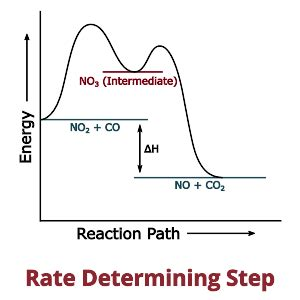
\includegraphics[height=0.8\textheight]{images/rate_determining_step.png}


\note{Det långsammaste steget i reaktionsmekanismen begränsar den totala reaktionshastigheten. Det har den högsta aktiveringsenergin och styr hur snabbt hela reaktionen fortlöper}
\end{frame}

% --- Slide 2: Flaskhalsar i lärande ---
\begin{frame}{Flaskhalsar i lärande}
Samma princip i utbildning: hitta flaskhalsen som begränsar hur snabbt du kan bli mer kvalificerad.

\begin{itemize}
    \item För kalkyl: grundläggande algebra
    \item För organisk kemi: molekylorbitalteori
\end{itemize}

Utbildningens struktur hjälper på makronivå, men för individuella kurser och din egen erfarenhet behöver du själv hitta dessa punkter.

\end{frame}

% --- Slide 3: Att upptäcka flaskhalsar ---
\begin{frame}{Att upptäcka flaskhalsar}
  \note{Det behöver heller inte ske aktiv, utan man lär sig väldigt snabbt att hitta detta}

Att identifiera flaskhalsar har aldrig varit ett problem för mig; jag tenderar att se det naturligt.
Därför kan jag inte ge det bästa råden om hur man upptäcker dem.

En del av detta löses av utbildningens struktur (t.ex. du lär dig inte biomolekyler innan du förstår molekyler).
\end{frame}

% --- Slide 4: Fyra metoder för övning ---
\begin{frame}{Fyra metoder för övning}
Scott Young beskriver fyra sätt att strukturera övning:
\begin{enumerate}
    \item Tidssegmentering: Isolera kritiska moment
    \item Kognitiva komponenter: Koppla bort överlappande färdigheter
    \item Härma: Replikera för att bemästra
    \item Förstoringsglasmetoden: Förstora svagheter
\end{enumerate}
\end{frame}

% --- Slide 5: Övning 1 ---
\begin{frame}{Övning 1: Tidssegmentering}
\begin{quote}
“Det enklaste sättet att skapa en övning är att isolera en tidssegment av en längre sekvens av handlingar.”\\
— Scott Young, \textit{Ultralearning}
\end{quote}

Exempel för bioteknik:
\begin{itemize}
    \item Pipettering
    \item Perfektionera grundläggande algebra innan kalkyl
    \item Förstå SN1- och SN2-substitution innan mekanismer
\end{itemize}
\end{frame}

% --- Slide 6: Övning 2 ---
\begin{frame}{Övning 2: Kognitiva komponenter}
Isolera en viss del av problemet och fokusera på det:
\begin{itemize}
    \item Markera det steg där du ofta misslyckas.
  \item För reaktionsmekanismer: förstå det svåraste steget först.
\note{Rita vattnets autoprotolys}
\end{itemize}
\end{frame}

% --- Slide 7: Övning 3 ---
\begin{frame}{Övning 3: Härma (replicera)}
\begin{quote}
“Genom att kopiera delar av färdigheten … kan du fokusera enbart på den komponent du vill öva.”\\
— Scott Young, \textit{Ultralearning}
\end{quote}

\begin{itemize}
    \item Använd mallar!
    \item Låt AI generera bakgrundsdelar
    \item Lägg all mental energi på det du faktiskt behöver lära dig
\end{itemize}
\end{frame}

% --- Slide 8: Övning 4 ---
\begin{frame}{Övning 4: Förstoringsglasmetoden}
\begin{quote}
“Spendera mer tid på en komponent av färdigheten än du annars skulle göra.”\\
— Scott Young, \textit{Ultralearning}
\end{quote}

Detta kan:
\begin{itemize}
    \item Minska din totala prestation
    \item Öka din inmatningstid
\end{itemize}

Men du spenderar en mycket större andel av din kognitiva energi på den svaghet du vill bemästra.
\end{frame}


% --- Slide 1: Intro ---
\begin{frame}{Ultralearning 4 – Förståelse och minne}
Detta är relevant för att studera inför tentor.\\[4pt]
För en djupare förståelse, läs \textit{Ultralearning}, kapitel~5.
\end{frame}

% --- Slide 2: Självtestning ---
\begin{frame}{Självtestning – hur du lär dig effektivt}
Du måste testa dig själv:

\begin{itemize}
    \item Förstå ett koncept: återberätta det med egna ord (otroligt effektivt)
    \item Mycket information: använd flashcards, helst skriv frågorna själv
    \item Användning av information: lös problem, särskilt tillämpade (se \textit{Urskilj detaljnivån})
    \item Mät förståelse: försök återkalla allt du vet om ämnet
\end{itemize}

\textbf{Tips:} Vänta med att kolla svaret --- kämpa lite först, det stärker minnet.
\end{frame}

% --- Slide 3: Iterera på svagheter ---
\begin{frame}{Iterera på svagheter}
Du kan alltid göra ett försök --- även om du inte känner dig redo.

\begin{itemize}
    \item Försök återkalla så mycket du kan
    \item Notera exakt vad som var svårt eller saknades
    \item Gör det till ett flashcard eller studera om just det momentet
\end{itemize}
\end{frame}

% --- Slide 4: Sömn och minne ---
\begin{frame}{Sömn och minne}
Information integreras i minnet när du sover.

\begin{itemize}
    \item Mer sömn → bättre konsolidering (upp till en viss gräns)
    \item Kvalitet och regelbundenhet är viktigare än kvantitet
\end{itemize}

För en djupare förståelse av neurologin, se:\\
\href{https://www.youtube.com/watch?v=ceFFEmkxTLg}{\textit{Neurologi och minne – videoinspelning}}
\end{frame}

% --- Slide 5: Långsiktigt minne ---
\begin{frame}{Långsiktigt minne}
Skolsystemet hjälper ofta genom introduktionsföreläsningar som repeterar tidigare material.

\begin{itemize}
  \item Använd digitala anteckningar (t.ex. Obsidian) för lättare repetition
  \item Pappersanteckningar fastnar bättre, så under \textit{Övning}, föredra det.
  \item Mycket behöver inte kommas ihåg permanent, var beredd att återlära äldre information vid behov
\end{itemize}
\end{frame}

% --- Slide 6: Personligt exempel ---
\begin{frame}{Personligt exempel}
Jag har använt flashcards för de flesta kurser.

\begin{itemize}
    \item Skapar kortlekar per föreläsning
    \item Associerar plats och kontext till varje koncept
    \item Jag har fortfarande levande bilder av föreläsningar kopplade till specifika idéer
\end{itemize}
\end{frame}

\begin{frame}{Ultralearning 5 - Intuition}
  \textbf{Intuition}
  \\
  För en djupare förståelse, läs \textit{Ultralearning}, kapitel 8.
  \\
  Att bygga intuition är syftet med din utbildning: om du förstår grunderna kommer du att kunna tillämpa dem. Du kan inte börja baklänges, då kommer du bara att lära dig läroboksexempel.
  \\
  \begin{quote}
  \small "När vi försöker lösa problem försöker vi ofta följa metoder eller en specifik väg bara för att de är de konventionella sätten. Men är de bäst? Tänkande från första principer tar bort antaganden och lämnar dig med endast en uppsättning fakta och ett önskat resultat. Därifrån kan du skapa din egen lösning."\\
  — Peter Hollins, \textit{Mental Models}
  \end{quote}
\end{frame}

\begin{frame}{Utförlig guide 5 - Intuition}
  Detta är varför du bör vara försiktig med att använda AI, bara studera tentafrågor eller lita på dina gruppmedlemmar. Om du inte lär dig är din utbildning förgäves.
  \\
  Hur vet du om du har intuition eller inte? Ställ dig själv många frågor.
\end{frame}

\begin{frame}{Feynman-tekniken}
  \textbf{Procedur:}
  \begin{enumerate}
    \item Skriv ner konceptet eller problemet du vill förstå.
    \item Förklara idén som om du skulle lära ut den till någon annan.
    \begin{itemize}
      \item Om det är ett koncept, förmedla idén till någon som aldrig har hört talas om det.
      \item Om det är ett problem, förklara hur man löser det och varför lösningen är logisk för dig.
    \end{itemize}
    \item När du fastnar, gå tillbaka till källmaterialet för att hitta svaret.
  \end{enumerate}
\end{frame}

\begin{frame}{Ett levande exempel - Språk}
\textbf{Grunderna:}
\begin{itemize}
\item Morfem → ord
\item Ord → sammansatta ord
\item Sammansatta ord → koncept
\item Utan grunder: memorera ord istället för idéer
\end{itemize}
\textbf{Illustrerande exempel:}
\begin{itemize}
\item Morfem: "foto" (ljus) + "syntes" (sammanställning/skapande)
\item Ord: "fotosyntes" (ljus-skapande, dvs. processen där ljus omvandlas till kemisk energi)
\item Sammansatta ord: "fotosyntesreaktion" (en specifik reaktion inom fotosyntes)
\item Koncept: Förstå hela processen med fotosyntes i biologi som helhet
\end{itemize}
\end{frame}

\begin{frame}{Exempel: Recombinant DNA}
  \textbf{Morfem:}
  \begin{itemize}
    \item Re-: igen / tillbaka
    \item Combine: förena
    \item -ant: som rör
    \item DNA: deoxiribonukleinsyra
  \end{itemize}
  Att förstå morfemen visar att "recombinant" betyder att kombinera igen.
\end{frame}

\begin{frame}{Exempel: Recombinant DNA (forts.)}
  \textbf{Ord och sammansatta ord:}
  \begin{itemize}
    \item Rekombinant DNA: DNA som har kombinerats artificiellt från olika källor.
  \end{itemize}
  \textbf{Koncept:}
  \begin{itemize}
    \item Används för att skapa nya genetiska sekvenser i bioteknik.
    \item Grundläggande för genteknik, genterapi, biofarmaceutiska läkemedel.
  \end{itemize}
\end{frame}

\begin{frame}{Att börja utan grunder}
  Om du börjar med konceptet utan att förstå ursprunget:
  \begin{itemize}
    \item Memorera fraser utan förståelse.
    \item Exempel: veta att recombinant DNA producerar insulin, men inte förstå hur.
  \end{itemize}
\end{frame}

\begin{frame}{Lära sig nya ord}
  \begin{itemize}
    \item Förbättra ordförråd genom att läsa.
    \item Fråga AI om ordens morfem och etymologi.
    \item Lär genom att använda. Se \textit{Urskilj detaljnivån}.
  \end{itemize}
\end{frame}

\begin{frame}{Stavning och språkval}
  \textbf{Stavning:}
  \begin{itemize}
    \item Skriv ner ord du stavar fel
    \item Öva dem tills de sitter
    \item Obsidian kan användas som digital ordbok
  \end{itemize}
  \textbf{Engelska eller svenska?}
  \begin{itemize}
    \item Det mesta materialet är på engelska
    \item Behöver förstå engelska för kurser och arbete
    \item (Majoriteten av presentationen är översatt m.h.a. AI)
  \end{itemize}
\end{frame}

\begin{frame}{Anteckningar}
  \textbf{Min syn på anteckningar:} \\
  Återkommande tema: hitta din egen metod och filosofi.

  Jag föredrar effektivitet och nöje för mina studier: jag gör det jag behöver snabbt, men låter det ta så lång tid som det krävs.

  \note{Du behöver inte dela min studiefilosofi, men jag är ganska nöjd med den och på tentorna är jag sällan besviken}

  \textbf{Zettelkasten:} \\
  Mitt tillvägagångssätt för studier och anteckningar är inte perfekt, men det följer min filosofi. Metoden utvecklades av Niklas Luhmann (1927–1998). Den hjälper dig att koppla idéer mellan olika områden och stimulera kreativt tänkande. Använd program som Obsidian. \\
  \textbf{Hur fungerar den?} \\
  Fragmentera anteckningarna så mycket som möjligt. Se separata anteckningar för detaljer och referera från huvudanteckningen. \\

\end{frame}

  \begin{frame}{Parkinson's law of triviality}

   \begin{figure}
    \centering
    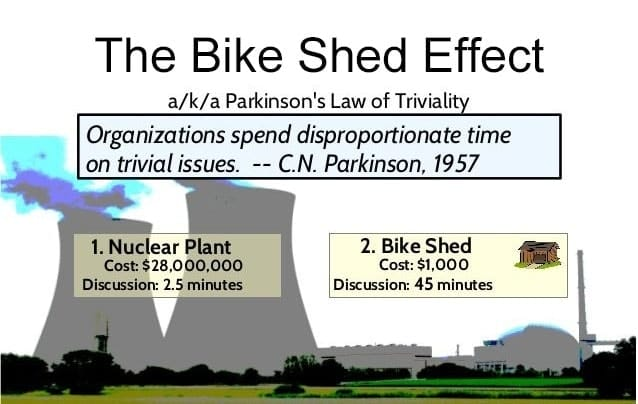
\includegraphics[width=0.7\linewidth]{images/bike_shed_effect.png}
  \end{figure}

   \note{Diskussion om kärnkraftverk vs cykelskjul. Små, enkla saker får oproportionerligt mycket uppmärksamhet}

  \textbf{Perfektion är prokrastinering:} \\
  Målet är att lära sig, inte att skapa perfekta anteckningar. Gör inte anteckningarna snygga, använd digitala anteckningar och skriv inte ner allt.
\end{frame}

  \begin{frame}{Anteckningar forts.}
  \textbf{Föreläsningar:} \\
  Lyssna aktivt. Skriv bara anteckningar på viktiga koncept. Materialet finns ofta redan i kurslitteratur och slides. Exempel på oväsentligt: ritningar, alla detaljer i reaktionsmekanismer, alla ekvationer. \\
  \textbf{Pappersbaserat eller digitalt?} \\
  Handanteckningar är bra för ekvationer och mekanismer, men digitala anteckningar är snabbare och mer tillgängliga. Spara viktiga exempel för flashcards.

  Några exempel värda att spara:
  \begin{itemize}
    \item kinetik
    \item Gibbs fria energi
    \item pH
    \item integraler
    \item statistiska koncept
\end{itemize}
\end{frame}

\section{Mjukvara}
\note{Fråga om deras erfarenhet med datorer och dylikt}
\begin{frame}{Mjukvaror}
  \textbf{Tre punkter om teknik och datorer:}
  \begin{itemize}
    \item Du kan inte vara rädd eller intala dig att du inte kan göra detta bara för att du studerar bioteknik.
    \item Ju bättre du kan datorer och hanterar dina filer, desto lättare blir livet.
    \item Du kommer behöva använda maskiner i arbetsmiljön, att förstå dem är nödvändigt. Minimum:
      \begin{itemize}
        \item Lär dig hur filer och filformat fungerar.
        \item Organisera filer, använd korrekta filnamn och säkerhetskopiera data.
      \end{itemize}
  \end{itemize}
  Ju tidigare du lär dig, desto bättre. Det bästa sättet är att förstå datorer från grunden; experimentera t.ex. med Linux.

\end{frame}

\begin{frame}{Mjukvaror}

  \textbf{Utmärkta mjukvaror:}
  \begin{itemize}
\item Obsidian: anteckningar, kombineras med Zettelkasten. Bra för att organisera kursmaterial och projektidéer.
\item LaTeX: skriva textdokument, rapporter, artiklar och uppsatser; standard inom akademisk publicering.
\item Zotero: hantera referenser och vetenskapliga artiklar; användbart vid litteraturöversikter.
\item Vim-bindings: effektiv text- och kodredigering; kan anpassas för olika språk och miljöer.
\item Emacs: kraftfull texteditor med stöd för anteckningar, programmering och integration med olika verktyg.
\item Git(hub): versionshantering av kod och projekt; viktigt för samarbete och spårning av förändringar.

  \end{itemize}
\end{frame}

\begin{frame}{AI eller inte AI? --- Lita på intuition!}

  \textbf{Frågor att ställa:}
  \begin{itemize}
    \item Kan du använda AI för detta nu och i framtiden?
    \item Producerar AI kvantitet eller kvalitet?
  \end{itemize}

  \textbf{Problem med AI:}
  \begin{itemize}
    \item Beroende och lathet.
    \item Hallucinationer – falsk information.
  \end{itemize}

  \textbf{Det dåliga:}
  \begin{itemize}
    \item Kodning: AI kan skriva bättre, men du förstår kanske inte koden.
    \item Skrivuppgifter: risk för falsk information, kontrollera alltid.
  \end{itemize}

  \textbf{Det bra:}
  \begin{itemize}
    \item Manuellt arbete: effektivitet.
    \item Tolka information: hjälp med grunder och statistik.
    \item Beskriva koncept: AI kan förklara, men verifiera.
    \item Få kritik: AI kan ge insikter, men kontrollera själv.
  \end{itemize}
\end{frame}

\begin{frame}{Avslutning}

  Ladda ned presentationen

  \textbf{Kontaktuppgifter:}
  \begin{itemize}
    \item \href{https://www.linkedin.com/in/rasmus-sten-788648235/}{LinkedIn}
    \item \href{mailto:rasmussten@hotmail.se}{rasmussten@hotmail.se}
  \end{itemize}

\end{frame}


\end{document}
